\documentclass[11pt,aspectratio=169]{beamer}
\usetheme{Madrid}

% ======================= PACKAGES =======================
\usepackage{graphicx}
\usepackage{booktabs}
\usepackage{adjustbox}
\usepackage{multicol}
\usepackage{amsmath}
\usepackage{amssymb}
\usepackage{tikz}
\usetikzlibrary{arrows,shapes,positioning,shadows,trees}
\usepackage{listings}
\usepackage{xcolor}

% ======================= COLOR DEFINITIONS =======================
% Primary color scheme: Blue/Teal for Digital Finance
\definecolor{dfblue}{RGB}{0,102,204}
\definecolor{dfteal}{RGB}{0,153,153}
\definecolor{dfcyan}{RGB}{51,187,204}
\definecolor{dflightblue}{RGB}{153,204,255}
\definecolor{dflightblue2}{RGB}{173,214,255}
\definecolor{dflightblue3}{RGB}{193,224,255}
\definecolor{dflightblue4}{RGB}{213,234,255}

% Accent colors for finance applications
\definecolor{dfgreen}{RGB}{44, 160, 44}
\definecolor{dfred}{RGB}{214, 39, 40}
\definecolor{dforange}{RGB}{255, 127, 14}
\definecolor{dfgray}{RGB}{127, 127, 127}

% Utility colors
\definecolor{lightgray}{RGB}{240, 240, 240}
\definecolor{midgray}{RGB}{180, 180, 180}
\definecolor{codebg}{RGB}{245, 245, 245}

% ======================= THEME CUSTOMIZATION =======================
% Apply Digital Finance color scheme to Madrid theme
\setbeamercolor{palette primary}{bg=dflightblue3,fg=dfblue}
\setbeamercolor{palette secondary}{bg=dflightblue2,fg=dfblue}
\setbeamercolor{palette tertiary}{bg=dfteal,fg=white}
\setbeamercolor{palette quaternary}{bg=dfblue,fg=white}

\setbeamercolor{structure}{fg=dfblue}
\setbeamercolor{section in toc}{fg=dfblue}
\setbeamercolor{subsection in toc}{fg=dfteal}
\setbeamercolor{title}{fg=dfblue}
\setbeamercolor{frametitle}{fg=dfblue,bg=dflightblue3}
\setbeamercolor{block title}{bg=dflightblue2,fg=dfblue}
\setbeamercolor{block body}{bg=dflightblue4,fg=black}

% Remove navigation symbols for cleaner look
\setbeamertemplate{navigation symbols}{}

% Clean itemize/enumerate
\setbeamertemplate{itemize items}[circle]
\setbeamertemplate{enumerate items}[default]

% Margins for readability
\setbeamersize{text margin left=8mm,text margin right=8mm}

% ======================= LISTINGS CONFIGURATION =======================
% Python code style
\lstdefinestyle{pythonstyle}{
    language=Python,
    basicstyle=\ttfamily\footnotesize,
    keywordstyle=\color{dfblue}\bfseries,
    stringstyle=\color{dforange},
    commentstyle=\color{dfgray}\itshape,
    numberstyle=\tiny\color{dfgray},
    numbers=left,
    numbersep=5pt,
    backgroundcolor=\color{codebg},
    showspaces=false,
    showstringspaces=false,
    showtabs=false,
    frame=single,
    rulecolor=\color{midgray},
    tabsize=4,
    captionpos=b,
    breaklines=true,
    breakatwhitespace=false,
    escapeinside={(*@}{@*)},
    xleftmargin=10pt,
    xrightmargin=10pt
}

% Solidity code style
\lstdefinestyle{soliditystyle}{
    language=Java, % closest approximation
    basicstyle=\ttfamily\footnotesize,
    keywordstyle=\color{dfteal}\bfseries,
    stringstyle=\color{dforange},
    commentstyle=\color{dfgray}\itshape,
    numberstyle=\tiny\color{dfgray},
    numbers=left,
    numbersep=5pt,
    backgroundcolor=\color{codebg},
    showspaces=false,
    showstringspaces=false,
    showtabs=false,
    frame=single,
    rulecolor=\color{midgray},
    tabsize=2,
    captionpos=b,
    breaklines=true,
    breakatwhitespace=false,
    escapeinside={(*@}{@*)},
    xleftmargin=10pt,
    xrightmargin=10pt,
    morekeywords={pragma, contract, function, returns, public, private, view, pure, payable, address, uint256, mapping, event, modifier}
}

% Inline code command
\newcommand{\code}[1]{\texttt{\color{dfblue}#1}}

% ======================= CUSTOM COMMANDS =======================
% Bottom annotation (Madrid-style)
\newcommand{\bottomnote}[1]{%
\vfill
\vspace{-2mm}
\textcolor{dflightblue2}{\rule{\textwidth}{0.4pt}}
\vspace{1mm}
\footnotesize
\textbf{#1}
}

% Compact list spacing
\newcommand{\compactlist}{%
\setlength{\itemsep}{0pt}%
\setlength{\parskip}{0pt}%
\setlength{\parsep}{0pt}%
}

% Chart placeholder
\newcommand{\chartplaceholder}[2][5cm]{%
\begin{center}
\begin{adjustbox}{max width=0.95\textwidth, max height=#1}
\framebox[\textwidth][c]{%
\rule{0pt}{#1}%
\textcolor{midgray}{[#2]}%
}
\end{adjustbox}
\end{center}
}

% ======================= FINANCE NOTATION MACROS =======================
% Probability and statistics
\newcommand{\E}{\mathbb{E}} % Expected value
\newcommand{\Var}{\mathrm{Var}} % Variance
\newcommand{\Cov}{\mathrm{Cov}} % Covariance
\newcommand{\Prob}{\mathbb{P}} % Probability

% Distributions
\newcommand{\Normal}{\mathcal{N}} % Normal distribution
\newcommand{\Uniform}{\mathcal{U}} % Uniform distribution

% Returns and prices
\newcommand{\Ret}{R} % Return
\newcommand{\LogRet}{r} % Log return
\newcommand{\Price}{S} % Price/Stock price
\newcommand{\Strike}{K} % Strike price

% Options and derivatives
\newcommand{\CallPrice}{C} % Call option price
\newcommand{\PutPrice}{P} % Put option price
\newcommand{\Greeks}[1]{\mathit{#1}} % Greek letters

% Risk measures
\newcommand{\VaR}{\mathrm{VaR}} % Value at Risk
\newcommand{\CVaR}{\mathrm{CVaR}} % Conditional VaR
\newcommand{\Sharpe}{\mathrm{SR}} % Sharpe Ratio

% Time series
\newcommand{\AR}{\mathrm{AR}} % Autoregressive
\newcommand{\MA}{\mathrm{MA}} % Moving average
\newcommand{\GARCH}{\mathrm{GARCH}} % GARCH

% Blockchain/Crypto
\newcommand{\Hash}{\mathrm{Hash}} % Hash function
\newcommand{\Block}{\mathcal{B}} % Block
\newcommand{\Chain}{\mathcal{C}} % Chain

% Real numbers, integers
\newcommand{\R}{\mathbb{R}}
\newcommand{\Z}{\mathbb{Z}}
\newcommand{\N}{\mathbb{N}}

% ======================= TIKZ STYLES =======================
% Styles for finance-related diagrams
\tikzstyle{process} = [rectangle, minimum width=3cm, minimum height=1cm, text centered, draw=dfblue, fill=dflightblue4, thick]
\tikzstyle{decision} = [diamond, minimum width=3cm, minimum height=1cm, text centered, draw=dfteal, fill=dflightblue4, thick]
\tikzstyle{arrow} = [thick,->,>=stealth,color=dfblue]
\tikzstyle{blockchain} = [rectangle, rounded corners, minimum width=2.5cm, minimum height=1cm, text centered, draw=dfteal, fill=dflightblue3, thick]
\tikzstyle{transaction} = [circle, minimum size=0.8cm, text centered, draw=dforange, fill=dflightblue4, thick]

% ======================= FOOTER TEMPLATE =======================
\setbeamertemplate{footline}{
    \hbox{\begin{beamercolorbox}[wd=\paperwidth,ht=2.5ex,dp=1ex,leftskip=.5em,rightskip=.5em]{author in head/foot}
    \tiny
    \textbf{Digital Finance} \hfill
    Joerg Osterrieder \hfill
    \insertdate \hfill
    Page \insertframenumber{} / \inserttotalframenumber
    \end{beamercolorbox}}
}

% ======================= SECTION DIVIDER TEMPLATE =======================
\AtBeginSection[]{
\begin{frame}[plain]
\vfill
\centering
\begin{beamercolorbox}[sep=12pt,center]{title}
\usebeamerfont{title}\LARGE\insertsection\par
\end{beamercolorbox}
\vfill
\end{frame}
}


% ======================= DOCUMENT INFO =======================
\title{Topic 5.3: DAO Governance}
\subtitle{Decentralized Autonomous Organizations}
\author{Joerg Osterrieder}
\institute{Digital Finance}
\date{2025}

\begin{document}

% =====================================================================
% SLIDE 1: Title Slide
% =====================================================================
\begin{frame}[plain]
\titlepage
\end{frame}

% =====================================================================
% SLIDE 2: Learning Objectives
% =====================================================================
\begin{frame}{Learning Objectives}
\begin{columns}[T]
\begin{column}{0.55\textwidth}
\textbf{By the end of this topic, you will be able to:}
\begin{enumerate}
\item Explain DAO governance mechanisms and their tradeoffs
\item Identify governance attack vectors and defenses
\item Evaluate tradeoffs between on-chain and off-chain governance
\item Understand why ``code is law'' is insufficient
\item Analyze token distribution's impact on voting power
\end{enumerate}
\end{column}
\begin{column}{0.42\textwidth}
\begin{block}{Core Question}
Can decentralized organizations achieve effective governance without central authority?
\end{block}

\vspace{3mm}
\textbf{Key Insight:}\\
Governance IS the attack surface. Secure code means nothing if governance can change it.
\end{column}
\end{columns}
\end{frame}

% =====================================================================
% SLIDE 3: Prerequisites  [C12, C14, C15 FIXED]
% =====================================================================
\begin{frame}{Prerequisites and Background}
\begin{columns}[T]
\begin{column}{0.48\textwidth}
\textbf{What You Should Already Know:}
\begin{itemize}
\item Basic blockchain concepts (from Days 1--3)
\item Smart contract fundamentals (from T5.1)
\item DeFi protocol basics (from T5.2)
\end{itemize}

\vspace{3mm}
\textbf{No Prior Knowledge Needed For:}
\begin{itemize}
\item Voting systems --- we explain everything from scratch
\item Game theory --- we introduce concepts as we go
\item Square root calculations --- we walk through every example
\end{itemize}
\end{column}
\begin{column}{0.48\textwidth}
\textbf{Conceptual Foundations:}
\begin{itemize}
\item Traditional corporate governance (boards, shareholders)
\item Democratic voting systems (elections, referendums)
\item The challenge of making sure the people who manage an organization actually serve the members' interests, not their own
\end{itemize}

\vspace{3mm}
\begin{alertblock}{Important Context}
DAOs attempt to solve the coordination problem: How can groups make collective decisions without trusted intermediaries?
\end{alertblock}
\end{column}
\end{columns}
\end{frame}

% =====================================================================
% SLIDE 4: Historical Context  [H42 FIXED]
% =====================================================================
\begin{frame}{Historical Context: The DAO}
\begin{columns}[T]
\begin{column}{0.55\textwidth}
\textbf{The Original DAO (2016):}
\begin{itemize}
\item First major DAO experiment on Ethereum
\item Raised \$150M in crowdfunding
\item Hacker exploited reentrancy vulnerability\\
      {\footnotesize (Recall from T5.1: reentrancy = the bug where a contract can be tricked into sending money multiple times before updating its records)}
\item Drained \$60M from the fund
\item Led to Ethereum/Ethereum Classic split
\end{itemize}

\vspace{3mm}
\textbf{Key Lesson:}\\
The ``code is law'' philosophy was tested---and the community chose human intervention over code finality.
\end{column}
\begin{column}{0.42\textwidth}
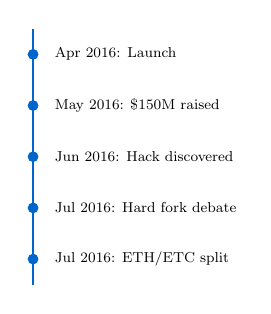
\begin{tikzpicture}[scale=0.65, transform shape]
% Timeline
\draw[thick, dfblue] (0,0) -- (0,5);

% Events
\node[right, font=\footnotesize] at (0.3,4.5) {Apr 2016: Launch};
\node[right, font=\footnotesize] at (0.3,3.5) {May 2016: \$150M raised};
\node[right, font=\footnotesize] at (0.3,2.5) {Jun 2016: Hack discovered};
\node[right, font=\footnotesize] at (0.3,1.5) {Jul 2016: Hard fork debate};
\node[right, font=\footnotesize] at (0.3,0.5) {Jul 2016: ETH/ETC split};

% Dots
\foreach \y in {0.5,1.5,2.5,3.5,4.5}
    \fill[dfblue] (0,\y) circle (3pt);
\end{tikzpicture}
\end{column}
\end{columns}
\end{frame}

% =====================================================================
% SLIDE 5: What is a DAO?  [C17 FIXED --- real-world analogy added]
% =====================================================================
\begin{frame}{What is a DAO?}
\begin{columns}[T]
\begin{column}{0.48\textwidth}
\textbf{Decentralized Autonomous Organization:}
\begin{itemize}
\item Rules encoded in smart contracts
\item Decisions via token holder voting
\item Treasury managed on-chain
\item No traditional legal structure
\item ``Code is law'' philosophy
\end{itemize}

\vspace{3mm}
\textbf{Analogy:} Imagine a club where:
\begin{enumerate}
\item The rules are written in a contract that nobody can secretly change
\item Every member votes on decisions using tokens instead of raised hands
\item The treasury is managed by code, not a treasurer who could run away with the money
\end{enumerate}
That's a DAO.
\end{column}
\begin{column}{0.48\textwidth}
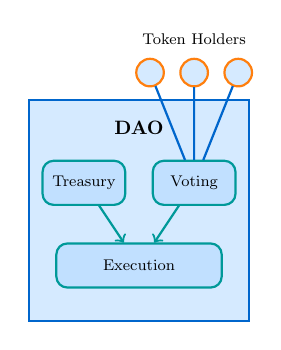
\begin{tikzpicture}[scale=0.7, transform shape]
% DAO structure
\draw[thick, dfblue, fill=dflightblue4] (0,0) rectangle (4,4);
\node at (2,3.5) {\textbf{DAO}};

% Components
\node (treasury) [blockchain, minimum width=1.5cm, minimum height=0.8cm] at (1,2.5) {\footnotesize Treasury};
\node (voting) [blockchain, minimum width=1.5cm, minimum height=0.8cm] at (3,2.5) {\footnotesize Voting};
\node (exec) [blockchain, minimum width=3cm, minimum height=0.8cm] at (2,1) {\footnotesize Execution};

\draw[->, thick, dfteal] (voting) -- (exec);
\draw[->, thick, dfteal] (treasury) -- (exec);

% Token holders
\node (h1) [transaction, above of=voting, node distance=2cm, minimum size=0.5cm] {};
\node (h2) [transaction, left of=h1, node distance=0.8cm, minimum size=0.5cm] {};
\node (h3) [transaction, right of=h1, node distance=0.8cm, minimum size=0.5cm] {};

\draw[thick, dfblue] (h1) -- (voting);
\draw[thick, dfblue] (h2) -- (voting);
\draw[thick, dfblue] (h3) -- (voting);

\node[above of=h1, node distance=0.6cm, font=\footnotesize] {Token Holders};
\end{tikzpicture}
\end{column}
\end{columns}
\end{frame}

% =====================================================================
% SLIDE 6: DAO Components
% =====================================================================
\begin{frame}{Core DAO Components}
\begin{center}
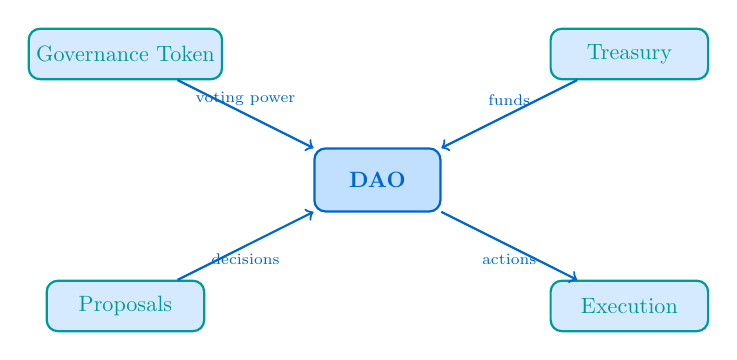
\begin{tikzpicture}[scale=0.8, transform shape]
% Central DAO
\node[draw, thick, dfblue, fill=dflightblue3, minimum width=2cm, minimum height=1cm, rounded corners] (dao) at (0,0) {\textbf{DAO}};

% Components around
\node[draw, thick, dfteal, fill=dflightblue4, minimum width=2.5cm, minimum height=0.8cm, rounded corners] (token) at (-4,2) {Governance Token};
\node[draw, thick, dfteal, fill=dflightblue4, minimum width=2.5cm, minimum height=0.8cm, rounded corners] (treasury) at (4,2) {Treasury};
\node[draw, thick, dfteal, fill=dflightblue4, minimum width=2.5cm, minimum height=0.8cm, rounded corners] (proposals) at (-4,-2) {Proposals};
\node[draw, thick, dfteal, fill=dflightblue4, minimum width=2.5cm, minimum height=0.8cm, rounded corners] (execution) at (4,-2) {Execution};

% Arrows
\draw[->, thick, dfblue] (token) -- (dao) node[midway, above, font=\scriptsize] {voting power};
\draw[->, thick, dfblue] (treasury) -- (dao) node[midway, above, font=\scriptsize] {funds};
\draw[->, thick, dfblue] (proposals) -- (dao) node[midway, below, font=\scriptsize] {decisions};
\draw[->, thick, dfblue] (dao) -- (execution) node[midway, below, font=\scriptsize] {actions};
\end{tikzpicture}
\end{center}

\vspace{3mm}
\begin{columns}[T]
\begin{column}{0.48\textwidth}
\textbf{Governance Token:} Represents voting power and economic stake in the protocol
\end{column}
\begin{column}{0.48\textwidth}
\textbf{Treasury:} Pooled funds controlled by governance votes, often billions in value
\end{column}
\end{columns}
\end{frame}

% =====================================================================
% SLIDE 7: Token-Based Voting  [H45 FIXED --- shareholder analogy added]
% =====================================================================
\begin{frame}{Token-Based Voting (1 Token = 1 Vote)}
\begin{columns}[T]
\begin{column}{0.48\textwidth}
\textbf{How It Works:}
\begin{itemize}
\item Each token equals one vote
\item Simple and transparent
\item Aligns voting with economic stake
\item Most common mechanism
\end{itemize}

\vspace{2mm}
\textbf{Analogy:} Token voting works like corporate shareholder voting: 1 share = 1 vote. If you own more shares (tokens), you have more say. Simple, but this creates a problem\ldots

\vspace{2mm}
\textbf{Example:}\\
If you hold 100 tokens out of 1,000,000 total, you have 0.01\% voting power.
\end{column}
\begin{column}{0.48\textwidth}
\textbf{Advantage:}\\
Economic skin in the game---those most invested have most say.

\vspace{3mm}
\textbf{Disadvantage:}\\
Wealth equals power---by design. This is the \textbf{plutocracy problem}, and it is the central challenge of DAO governance.

\vspace{3mm}
\begin{alertblock}{Critical Issue}
If 10 wallets hold 60\% of tokens, democracy becomes oligarchy. The majority of token holders have no meaningful voice.
\end{alertblock}
\end{column}
\end{columns}
\end{frame}

% =====================================================================
% SLIDE 8: The Plutocracy Problem  [H47 FIXED --- moved BEFORE solutions]
% =====================================================================
\begin{frame}{The Plutocracy Problem}
\begin{center}
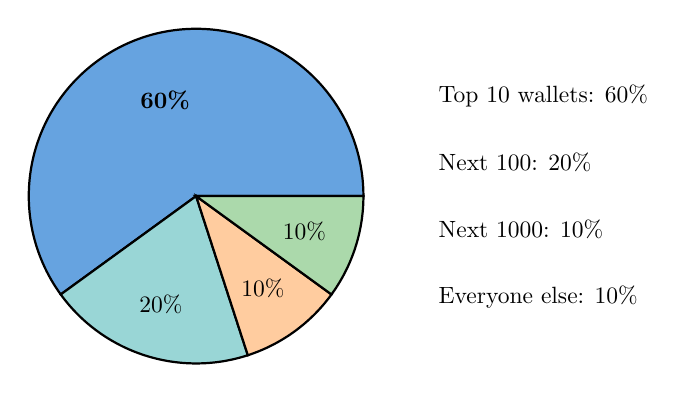
\begin{tikzpicture}[scale=0.85, transform shape]
% Token distribution pie chart
\draw[thick, fill=dfblue!60] (0,0) -- (0:2.5) arc (0:216:2.5) -- cycle;
\draw[thick, fill=dfteal!40] (0,0) -- (216:2.5) arc (216:288:2.5) -- cycle;
\draw[thick, fill=dforange!40] (0,0) -- (288:2.5) arc (288:324:2.5) -- cycle;
\draw[thick, fill=dfgreen!40] (0,0) -- (324:2.5) arc (324:360:2.5) -- cycle;

% Labels
\node at (108:1.5) {\textbf{60\%}};
\node at (252:1.7) {20\%};
\node at (306:1.7) {10\%};
\node at (342:1.7) {10\%};

% Legend
\node[right] at (3.5,1.5) {Top 10 wallets: 60\%};
\node[right] at (3.5,0.5) {Next 100: 20\%};
\node[right] at (3.5,-0.5) {Next 1000: 10\%};
\node[right] at (3.5,-1.5) {Everyone else: 10\%};
\end{tikzpicture}
\end{center}

\vspace{3mm}
\textbf{Reality:} Most DAOs have highly concentrated token distributions.\\
\textbf{Result:} A few whales control most decisions. ``Decentralized'' in name only.
\end{frame}

% =====================================================================
% SLIDE 9: Real DAO Concentration Data
% =====================================================================
\begin{frame}{Real-World Token Concentration}
\begin{center}
\textbf{Top 10 Holders' Share of Governance Tokens}

\vspace{3mm}
\begin{tabular}{|l|c|c|}
\hline
\textbf{DAO} & \textbf{Top 10 Share} & \textbf{Implication} \\
\hline
MakerDAO (MKR) & 48.2\% & Near majority control \\
\hline
Uniswap (UNI) & 52.1\% & Majority control \\
\hline
Compound (COMP) & 57.8\% & Strong majority \\
\hline
Aave (AAVE) & 42.3\% & Significant influence \\
\hline
Curve (CRV) & 61.5\% & Dominant control \\
\hline
\end{tabular}
\end{center}

\vspace{3mm}
\begin{alertblock}{Key Insight}
In most ``decentralized'' protocols, fewer than 10 entities can pass any proposal they want. This is not a bug---it reflects how token distributions naturally evolve.
\end{alertblock}
\end{frame}

% =====================================================================
% SLIDE 10: Why So Many Voting Systems?  [C16 FIXED --- motivation bridge]
% =====================================================================
\begin{frame}{Why So Many Voting Systems?}
\begin{columns}[T]
\begin{column}{0.48\textwidth}
\textbf{The Core Problem:}\\
Simple token voting (1 token = 1 vote) has a fatal flaw: it turns ``decentralized governance'' into rule by the wealthiest token holders.

\vspace{3mm}
\textbf{So researchers and developers have proposed alternatives.} Each tries to fix plutocracy in a different way:

\vspace{3mm}
\begin{block}{Basic (next two slides)}
\begin{itemize}
\item \textbf{Quadratic Voting} --- make extra votes increasingly expensive
\item \textbf{Conviction Voting} --- reward long-term commitment
\end{itemize}
\end{block}
\end{column}
\begin{column}{0.48\textwidth}
\begin{block}{Advanced (later slides)}
\begin{itemize}
\item \textbf{Delegation} --- let experts vote on your behalf
\item \textbf{Optimistic Governance} --- approve unless someone objects
\item \textbf{Multi-Sig} --- require multiple keyholders
\item \textbf{Futarchy} --- use prediction markets to decide
\end{itemize}
\end{block}

\vspace{3mm}
\begin{alertblock}{No Silver Bullet}
Every mechanism trades one problem for another. The art of DAO design is choosing the right combination.
\end{alertblock}
\end{column}
\end{columns}
\end{frame}

% =====================================================================
% SLIDE 11: Quadratic Voting  [H37, H40, C13 FIXED]
% =====================================================================
\begin{frame}{Quadratic Voting}
\begin{columns}[T]
\begin{column}{0.55\textwidth}
\textbf{Core Concept:}
$$\text{Voting Power} = \sqrt{\text{Tokens Held}}$$

\vspace{1mm}
\textbf{Why the square root?} It makes each additional vote on the same issue increasingly expensive. Your 1st vote costs 1 token. Your 2nd vote costs 4 tokens total. Your 3rd costs 9. This means a passionate minority can express strong preferences, but cannot simply buy dominance.

\vspace{2mm}
\textbf{Example Calculations:}
\begin{itemize}
\item 100 tokens $\rightarrow \sqrt{100} = 10$ votes
\item 10,000 tokens $\rightarrow \sqrt{10{,}000} = 100$ votes
\item 1,000,000 tokens $\rightarrow \sqrt{1{,}000{,}000} = 1{,}000$ votes
\end{itemize}

\vspace{1mm}
\textbf{Impact:}\\
A whale with 10,000x more tokens only gets 100x more votes (not 10,000x).
\end{column}
\begin{column}{0.42\textwidth}
\textbf{Advantages:}
\begin{itemize}
\item Reduces whale dominance
\item Gives small holders more voice
\item Encourages broader participation
\end{itemize}

\vspace{2mm}
\textbf{Critical Vulnerability:}
\begin{alertblock}{Sybil Attack}
A \textbf{Sybil attack} is when one person creates many fake identities to gain disproportionate influence (named after a book about multiple personalities).

\vspace{1mm}
\footnotesize
Under regular voting: 1 person, 100 tokens = 100 votes. Split into 10 wallets of 10 each = still 100 votes.\\[1mm]
Under quadratic voting: 1 person, 100 tokens = $\sqrt{100}=10$ votes. Split into 10 wallets: $10 \times \sqrt{10} \approx 31.6$ votes.\\[1mm]
\textbf{Splitting INCREASES power!} Quadratic voting requires identity verification.
\end{alertblock}
\end{column}
\end{columns}
\end{frame}

% =====================================================================
% SLIDE 12: Conviction Voting  [H38 FIXED --- worked example added]
% =====================================================================
\begin{frame}{Conviction Voting}
\begin{columns}[T]
\begin{column}{0.48\textwidth}
\textbf{How It Works:}
\begin{itemize}
\item Votes accumulate over time
\item Longer stake = more voting power
\item Rewards long-term alignment
\item Prevents flash loan attacks
\end{itemize}

\vspace{2mm}
\textbf{Worked Example} (decay factor = 0.9):\\
Alice stakes 100 tokens on Proposal A:
\begin{itemize}
\item Day 1: conviction = 100
\item Day 2: conviction = 190 $(100 + 90)$
\item Day 3: conviction = 271 $(190 + 81)$
\item Day 4: conviction = 344 $(271 + 73)$
\end{itemize}
Her conviction grows over time but at a decreasing rate. When total conviction crosses the threshold, the proposal passes.
\end{column}
\begin{column}{0.48\textwidth}
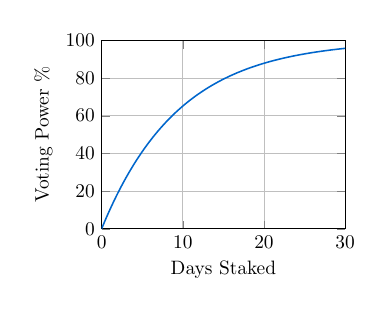
\begin{tikzpicture}[scale=0.7, transform shape]
\begin{axis}[
    xlabel={Days Staked},
    ylabel={Voting Power \%},
    xmin=0, xmax=30,
    ymin=0, ymax=100,
    grid=major,
    width=6cm,
    height=5cm
]
\addplot[domain=0:30, samples=100, thick, dfblue] {100*(1-0.9^x)};
\end{axis}
\end{tikzpicture}

\vspace{2mm}
\textbf{Tradeoff:}\\
Slower decision-making. Emergencies require alternative mechanisms.

\vspace{2mm}
\textbf{Difficulty:} \textit{Intermediate} --- requires understanding how time affects voting power.
\end{column}
\end{columns}
\end{frame}

% =====================================================================
% SLIDE 13: Delegation  [H35 FIXED --- liquid democracy explained]
% =====================================================================
\begin{frame}{Vote Delegation (Liquid Democracy)}
\begin{columns}[T]
\begin{column}{0.48\textwidth}
\textbf{What Is Liquid Democracy?}\\
In liquid democracy, you can either vote yourself OR delegate your vote to someone you trust---and take it back anytime. Think of it as a ``flexible proxy'' system.

\vspace{2mm}
\textbf{How Delegation Works:}
\begin{itemize}
\item Delegate votes to trusted experts
\item Retain token ownership
\item Can revoke delegation anytime
\item Addresses voter apathy
\end{itemize}

\vspace{2mm}
\textbf{Popular Implementations:}
\begin{itemize}
\item Compound Finance delegates
\item Uniswap governance
\item ENS DAO delegation
\end{itemize}
\end{column}
\begin{column}{0.48\textwidth}
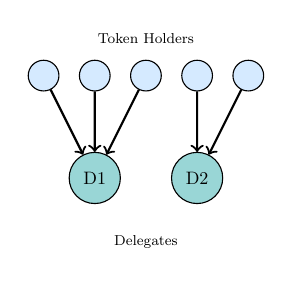
\begin{tikzpicture}[scale=0.65, transform shape]
% Small holders
\node[draw, circle, fill=dflightblue4, minimum size=0.6cm] (h1) at (0,3) {};
\node[draw, circle, fill=dflightblue4, minimum size=0.6cm] (h2) at (1,3) {};
\node[draw, circle, fill=dflightblue4, minimum size=0.6cm] (h3) at (2,3) {};
\node[draw, circle, fill=dflightblue4, minimum size=0.6cm] (h4) at (3,3) {};
\node[draw, circle, fill=dflightblue4, minimum size=0.6cm] (h5) at (4,3) {};

\node[above, font=\footnotesize] at (2,3.5) {Token Holders};

% Delegates
\node[draw, circle, fill=dfteal!40, minimum size=1cm] (d1) at (1,1) {D1};
\node[draw, circle, fill=dfteal!40, minimum size=1cm] (d2) at (3,1) {D2};

\node[below, font=\footnotesize] at (2,0) {Delegates};

% Arrows
\draw[->, thick] (h1) -- (d1);
\draw[->, thick] (h2) -- (d1);
\draw[->, thick] (h3) -- (d1);
\draw[->, thick] (h4) -- (d2);
\draw[->, thick] (h5) -- (d2);
\end{tikzpicture}

\vspace{2mm}
\begin{alertblock}{Risk}
Delegation can further concentrate power among a few prominent delegates.
\end{alertblock}
\end{column}
\end{columns}
\end{frame}

% =====================================================================
% SLIDE 14: Multi-Sig Governance  [H36 FIXED --- bank vault analogy]
% =====================================================================
\begin{frame}{Multi-Signature (Multi-Sig) Governance}
\begin{columns}[T]
\begin{column}{0.48\textwidth}
\textbf{Analogy:} Like a bank vault that needs 3 out of 5 keyholders to open. An N-of-M signature means N people (out of M total) must approve before a transaction goes through.

\vspace{3mm}
\textbf{N-of-M Signing:}
\begin{itemize}
\item N signers must approve out of M total
\item Example: 3-of-5 multi-sig
\item Fast execution for routine decisions
\item Common for treasury management
\end{itemize}

\vspace{3mm}
\textbf{Popular Tools:}
\begin{itemize}
\item Gnosis Safe (most common)
\item Aragon multi-sig
\item Custom implementations
\end{itemize}
\end{column}
\begin{column}{0.48\textwidth}
\textbf{Tradeoffs:}

\begin{tabular}{|l|c|}
\hline
\textbf{Aspect} & \textbf{Rating} \\
\hline
Speed & High \\
\hline
Decentralization & Low \\
\hline
Security & Medium \\
\hline
Transparency & Medium \\
\hline
\end{tabular}

\vspace{3mm}
\begin{block}{Common Pattern}
Many DAOs combine multi-sig for day-to-day operations with token voting for major decisions.
\end{block}
\end{column}
\end{columns}
\end{frame}

% =====================================================================
% SLIDE 15: Optimistic Governance  [H46 FIXED --- work analogy added]
% =====================================================================
\begin{frame}{Optimistic Governance}
\begin{columns}[T]
\begin{column}{0.48\textwidth}
\textbf{Analogy:} Like expense approvals at work: submit your receipt, and it is automatically approved UNLESS someone objects within 3 days. Most proposals pass without drama---only controversial ones get challenged.

\vspace{2mm}
\textbf{How It Works:}
\begin{enumerate}
\item Proposal submitted
\item Short challenge period begins
\item If no veto $\rightarrow$ auto-execute
\item If vetoed $\rightarrow$ standard vote
\end{enumerate}
\end{column}
\begin{column}{0.48\textwidth}
\textbf{Advantages:}
\begin{itemize}
\item Dramatically increases speed
\item Reduces voter fatigue
\item People only engage when they disagree
\end{itemize}

\vspace{3mm}
\textbf{Requirements:}
\begin{itemize}
\item Active community monitoring
\item Fast response capability
\item Clear veto thresholds
\end{itemize}

\vspace{2mm}
\begin{alertblock}{Best For}
Low-risk parameter changes, not major protocol upgrades.
\end{alertblock}
\end{column}
\end{columns}
\end{frame}

% =====================================================================
% SLIDE 16: Voting Mechanism Comparison  [C16 FIXED --- comparison table]
% =====================================================================
\begin{frame}{Voting Mechanism Comparison}
\begin{center}
\renewcommand{\arraystretch}{1.3}
\begin{tabular}{|l|c|c|c|c|}
\hline
\textbf{Mechanism} & \textbf{Whale-Proof?} & \textbf{Speed} & \textbf{Complexity} & \textbf{Identity Needed?} \\
\hline
Token Voting & No & Fast & Low & No \\
\hline
Quadratic & Partially & Fast & Medium & Yes \\
\hline
Conviction & Yes & Slow & Medium & No \\
\hline
Delegation & No & Fast & Low & No \\
\hline
Multi-Sig & N/A & Very Fast & Low & Yes \\
\hline
Optimistic & No & Very Fast & Low & No \\
\hline
\end{tabular}
\end{center}

\vspace{3mm}
\begin{columns}[T]
\begin{column}{0.48\textwidth}
\begin{block}{Key Takeaway}
No single mechanism solves all problems. Most successful DAOs combine multiple mechanisms for different types of decisions.
\end{block}
\end{column}
\begin{column}{0.48\textwidth}
\begin{alertblock}{Real-World Pattern}
Routine changes: optimistic or multi-sig.\\
Major upgrades: token voting with timelock.\\
Treasury grants: conviction or quadratic.
\end{alertblock}
\end{column}
\end{columns}
\end{frame}

% =====================================================================
% SLIDE 17: Governance Attack Vectors  [H41, H43, H34 FIXED]
% =====================================================================
\begin{frame}{Governance Attack Vectors}
\begin{columns}[T]
\begin{column}{0.48\textwidth}
\textbf{Flash Loan Governance Attack:}\\
{\footnotesize (Remember flash loans from T5.1: borrow millions instantly, use them, return them---all in one transaction.)}
\begin{enumerate}
\item Borrow millions in governance tokens
\item Vote on malicious proposal
\item Execute immediately
\item Repay loan, keep profits
\end{enumerate}

\vspace{2mm}
\textbf{Beanstalk Attack (2022):}
\begin{itemize}
\item Flash borrowed \$1B in tokens
\item Passed proposal in one block
\item Drained \$182M from treasury
\item All in a single transaction
\end{itemize}
\end{column}
\begin{column}{0.48\textwidth}
\textbf{Other Attack Vectors} (ranked by prevalence):
\begin{enumerate}
\item \textbf{Whale dominance} (every major DAO)---large holders outvote everyone else
\item \textbf{Voter apathy} (widespread)---too few people vote, making attacks easier
\item \textbf{Flash loan attacks} (rare but devastating)---borrow tokens, vote, return them
\item \textbf{Dark DAOs} (theoretical)---secret organizations that pay voters to vote a certain way, like a hidden lobby that bribes shareholders
\item \textbf{Governance capture} (emerging)---slowly accumulating enough power to control the protocol
\end{enumerate}
\end{column}
\end{columns}
\end{frame}

% =====================================================================
% SLIDE 18: Beanstalk Case Study
% =====================================================================
\begin{frame}{Case Study: Beanstalk Governance Attack}
\begin{center}
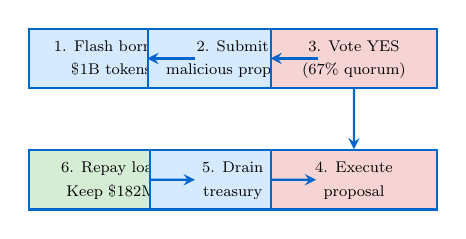
\begin{tikzpicture}[scale=0.7, transform shape, node distance=2.2cm]
% Attack sequence
\node (step1) [process, minimum width=3cm] {
\begin{tabular}{c}
\footnotesize 1. Flash borrow\\
\footnotesize \$1B tokens
\end{tabular}
};

\node (step2) [process, right of=step1, minimum width=3cm] {
\begin{tabular}{c}
\footnotesize 2. Submit\\
\footnotesize malicious proposal
\end{tabular}
};

\node (step3) [process, right of=step2, minimum width=3cm, fill=dfred!20] {
\begin{tabular}{c}
\footnotesize 3. Vote YES\\
\footnotesize (67\% quorum)
\end{tabular}
};

\node (step4) [process, below of=step1, minimum width=3cm, fill=dfgreen!20] {
\begin{tabular}{c}
\footnotesize 6. Repay loan\\
\footnotesize Keep \$182M
\end{tabular}
};

\node (step5) [process, below of=step2, minimum width=3cm] {
\begin{tabular}{c}
\footnotesize 5. Drain\\
\footnotesize treasury
\end{tabular}
};

\node (step6) [process, below of=step3, minimum width=3cm, fill=dfred!20] {
\begin{tabular}{c}
\footnotesize 4. Execute\\
\footnotesize proposal
\end{tabular}
};

\draw[arrow] (step1) -- (step2);
\draw[arrow] (step2) -- (step3);
\draw[arrow] (step3) -- (step6);
\draw[arrow] (step6) -- (step5);
\draw[arrow] (step5) -- (step4);
\end{tikzpicture}
\end{center}

\vspace{3mm}
\textbf{Critical flaw:} No time delay between vote and execution.\\
\textbf{Fix:} Timelocks, snapshot voting, flash loan protection.
\end{frame}

% =====================================================================
% SLIDE 19: Governance Defenses - Timelocks  [M5 FIXED --- analogy added]
% =====================================================================
\begin{frame}{Governance Defense: Timelocks}
\begin{columns}[T]
\begin{column}{0.48\textwidth}
\textbf{Analogy:} A timelock is a mandatory ``cooling-off period'' --- like the waiting period when you buy a house, giving you time to reconsider before the deal is final.

\vspace{2mm}
\textbf{How Timelocks Work:}
\begin{itemize}
\item Delay between approval and execution
\item Typically 24--72 hours minimum
\item Gives community time to react
\item Critical security mechanism
\end{itemize}

\vspace{2mm}
\textbf{Real Examples:}
\begin{itemize}
\item Uniswap: 7-day timelock
\item Compound: 48-hour timelock
\item MakerDAO: Variable by risk
\end{itemize}
\end{column}
\begin{column}{0.48\textwidth}
\textbf{What Happens During Timelock:}
\begin{enumerate}
\item Community reviews approved proposal
\item Users can exit protocol if they disagree
\item Guardians can cancel malicious proposals
\item Security researchers can alert issues
\end{enumerate}

\vspace{3mm}
\begin{block}{Tradeoff}
Longer timelock = more security but slower operations. Emergency situations require special mechanisms.
\end{block}
\end{column}
\end{columns}
\end{frame}

% =====================================================================
% SLIDE 20: Vote Escrow (veTokens)  [H39, M1 FIXED]
% =====================================================================
\begin{frame}{Vote Escrow: The veToken Model}
\begin{columns}[T]
\begin{column}{0.48\textwidth}
\textbf{Intuition:} veTokens are a ``commitment multiplier.'' Lock your tokens for longer, get more voting power. Lock for 1 year = 1x votes. Lock for 4 years = 4x votes. This rewards long-term commitment over short-term speculation.

\vspace{2mm}
\textbf{How veTokens Work:}
\begin{itemize}
\item Lock tokens to gain voting power
\item Longer lock = more voting power
\item Maximum lock often 4 years
\item Pioneered by Curve Finance
\end{itemize}

\vspace{2mm}
\textbf{Voting Power Formula:}
$$\text{vePower} = \text{Tokens} \times \frac{\text{Lock Time}}{\text{Max Lock}}$$

Example: 100 CRV locked 2 years\\
$= 100 \times \frac{2}{4} = 50$ veCRV
\end{column}
\begin{column}{0.48\textwidth}
\textbf{Why It Prevents Flash Loans:}
\begin{itemize}
\item Tokens must be locked to vote
\item Flash loans require same-block return
\item Cannot lock and unlock instantly
\item Attacker would need real capital
\end{itemize}

\vspace{3mm}
\textbf{Additional Benefits:}
\begin{itemize}
\item Aligns long-term incentives
\item Reduces token velocity (how quickly tokens change hands)
\item Committed stakeholders decide
\end{itemize}
\end{column}
\end{columns}
\end{frame}

% =====================================================================
% SLIDE 21: Snapshot Voting Defense
% =====================================================================
\begin{frame}{Snapshot Voting as Defense}
\begin{columns}[T]
\begin{column}{0.48\textwidth}
\textbf{How Snapshot Defense Works:}
\begin{itemize}
\item Record token balances at specific block
\item Block chosen BEFORE proposal created
\item Voting power based on historical balance
\item Flash loan has no effect
\end{itemize}

\vspace{3mm}
\textbf{Timeline:}
\begin{enumerate}
\item Block 100: Snapshot taken
\item Block 105: Proposal created
\item Block 150: Flash loan attempted
\item Result: Flash loan ignored---balance was 0 at block 100
\end{enumerate}
\end{column}
\begin{column}{0.48\textwidth}
\textbf{Implementation:}
\begin{itemize}
\item Snapshot.org (off-chain)
\item OpenZeppelin Governor (on-chain)
\item Custom snapshot contracts
\end{itemize}

\vspace{3mm}
\begin{block}{Key Insight}
Snapshot voting elegantly solves flash loan attacks without restricting token liquidity. Users can still trade freely---only historical balance matters for votes.
\end{block}
\end{column}
\end{columns}
\end{frame}

% =====================================================================
% SLIDE 22: Quorum Requirements  [M6 FIXED --- meeting analogy added]
% =====================================================================
\begin{frame}{Quorum Requirements}
\begin{columns}[T]
\begin{column}{0.48\textwidth}
\textbf{What is Quorum?}\\
\textbf{Analogy:} Like needing a minimum number of people at a meeting before you can take a valid vote. If too few show up, any decision is invalid.

\vspace{2mm}
\begin{itemize}
\item Minimum participation threshold
\item Vote invalid if quorum not met
\item Prevents minority rule
\item Typical range: 4--10\%
\end{itemize}

\vspace{2mm}
\textbf{Example:}\\
If quorum = 4\% and total supply = 1B tokens:\\
At least 40M tokens must vote for the result to be valid.
\end{column}
\begin{column}{0.48\textwidth}
\textbf{Higher Quorum for Critical Decisions:}

\begin{tabular}{|l|c|}
\hline
\textbf{Decision Type} & \textbf{Quorum} \\
\hline
Parameter change & 4\% \\
\hline
Treasury grant & 5\% \\
\hline
Protocol upgrade & 10\% \\
\hline
Emergency action & 15\% \\
\hline
\end{tabular}

\vspace{3mm}
\begin{alertblock}{The Quorum Dilemma}
Too low: Small group can pass anything\\
Too high: Nothing ever passes due to voter apathy
\end{alertblock}
\end{column}
\end{columns}
\end{frame}

% =====================================================================
% SLIDE 23: Guardian/Veto Power
% =====================================================================
\begin{frame}{Guardian and Veto Powers}
\begin{columns}[T]
\begin{column}{0.48\textwidth}
\textbf{Guardian Multi-Sig:}
\begin{itemize}
\item Small trusted group (5--9 members)
\item Can veto malicious proposals
\item ``Emergency brake'' function
\item Used during timelock period
\end{itemize}

\vspace{3mm}
\textbf{When Guardians Act:}
\begin{itemize}
\item Clear governance attack detected
\item Proposal would harm protocol
\item Bug discovered in approved code
\item Legal/regulatory emergency
\end{itemize}
\end{column}
\begin{column}{0.48\textwidth}
\textbf{The Centralization Tradeoff:}

\begin{center}
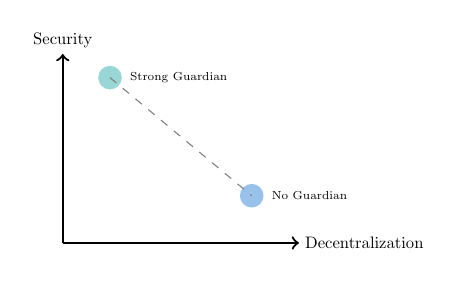
\begin{tikzpicture}[scale=0.6, transform shape]
\draw[->, thick] (0,0) -- (5,0) node[right] {Decentralization};
\draw[->, thick] (0,0) -- (0,4) node[above] {Security};

\node[fill=dfteal!40, circle, minimum size=0.5cm] at (1,3.5) {};
\node[right, font=\scriptsize] at (1.3,3.5) {Strong Guardian};

\node[fill=dfblue!40, circle, minimum size=0.5cm] at (4,1) {};
\node[right, font=\scriptsize] at (4.3,1) {No Guardian};

\draw[dashed, dfgray] (1,3.5) -- (4,1);
\end{tikzpicture}
\end{center}

\vspace{2mm}
\textbf{Best Practice:}\\
Sunset guardians over time as protocol matures and governance proves robust.
\end{column}
\end{columns}
\end{frame}

% =====================================================================
% SLIDE 24: Governance Lifecycle  [H48 FIXED --- new slide]
% =====================================================================
\begin{frame}{How a DAO Proposal Actually Works}
\begin{center}
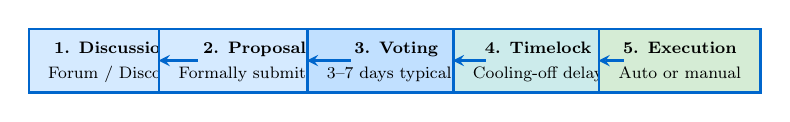
\begin{tikzpicture}[scale=0.75, transform shape, node distance=2.4cm]
\node (step1) [process, minimum width=2.5cm, fill=dflightblue4] {
\begin{tabular}{c}
\footnotesize \textbf{1. Discussion}\\
\footnotesize Forum / Discord
\end{tabular}
};

\node (step2) [process, right of=step1, minimum width=2.5cm, fill=dflightblue4] {
\begin{tabular}{c}
\footnotesize \textbf{2. Proposal}\\
\footnotesize Formally submitted
\end{tabular}
};

\node (step3) [process, right of=step2, minimum width=2.5cm, fill=dflightblue3] {
\begin{tabular}{c}
\footnotesize \textbf{3. Voting}\\
\footnotesize 3--7 days typically
\end{tabular}
};

\node (step4) [process, right of=step3, minimum width=2.5cm, fill=dfteal!20] {
\begin{tabular}{c}
\footnotesize \textbf{4. Timelock}\\
\footnotesize Cooling-off delay
\end{tabular}
};

\node (step5) [process, right of=step4, minimum width=2.5cm, fill=dfgreen!20] {
\begin{tabular}{c}
\footnotesize \textbf{5. Execution}\\
\footnotesize Auto or manual
\end{tabular}
};

\draw[arrow] (step1) -- (step2);
\draw[arrow] (step2) -- (step3);
\draw[arrow] (step3) -- (step4);
\draw[arrow] (step4) -- (step5);
\end{tikzpicture}
\end{center}

\vspace{3mm}
\begin{columns}[T]
\begin{column}{0.48\textwidth}
\textbf{Typical Timeline:}
\begin{itemize}
\item Discussion: 1--2 weeks on forums
\item Proposal: snapshot or on-chain submission
\item Voting: 3--7 day window
\item Timelock: 24 hours to 7 days
\item Execution: immediate (on-chain) or manual (off-chain)
\end{itemize}
\end{column}
\begin{column}{0.48\textwidth}
\textbf{Where Attacks Can Happen:}
\begin{itemize}
\item Step 2: Flash loan to create + vote instantly
\item Step 3: Vote buying during voting period
\item Step 4: This is where timelocks protect us
\item Step 5: Malicious code in proposal payload
\end{itemize}

\vspace{2mm}
\begin{block}{Key Point}
Each step is a potential point of failure---and a potential point of defense.
\end{block}
\end{column}
\end{columns}
\end{frame}

% =====================================================================
% SLIDE 25: On-Chain vs Off-Chain Governance
% =====================================================================
\begin{frame}{On-Chain vs. Off-Chain Governance}
\begin{center}
\renewcommand{\arraystretch}{1.3}
\begin{tabular}{|l|c|c|}
\hline
\textbf{Aspect} & \textbf{On-Chain} & \textbf{Off-Chain} \\
\hline
Binding & Automatic execution & Requires implementation \\
\hline
Transparency & Fully verifiable & Forum/snapshot \\
\hline
Cost & Gas fees & Usually free \\
\hline
Speed & Blockchain constrained & Faster iteration \\
\hline
Flexibility & Rigid (code) & Adaptable \\
\hline
Attacks & Flash loans, 51\% & Social, coordination \\
\hline
Examples & Compound, Uniswap & Bitcoin, Ethereum L1 \\
\hline
\end{tabular}
\end{center}

\vspace{3mm}
\begin{block}{Hybrid Approaches}
Most successful DAOs use both: off-chain discussion/signaling, on-chain execution with safeguards.
\end{block}
\end{frame}

% =====================================================================
% SLIDE 26: The Voter Apathy Problem  [L3 FIXED --- rational ignorance defined]
% =====================================================================
\begin{frame}{The Voter Apathy Problem}
\begin{columns}[T]
\begin{column}{0.55\textwidth}
\textbf{Reality of DAO Participation:}
\begin{itemize}
\item Typical turnout: 1--5\% of tokens
\item Most token holders never vote
\item Few wallets dominate decisions
\item Governance fatigue is real
\end{itemize}

\vspace{3mm}
\textbf{Why People Don't Vote:}
\begin{itemize}
\item Gas costs (on-chain)
\item Time to understand proposals
\item Rational ignorance---when the cost of learning about an issue exceeds the impact your single vote can have, it is ``rational'' to stay uninformed
\item Token holders $\neq$ users
\end{itemize}
\end{column}
\begin{column}{0.42\textwidth}
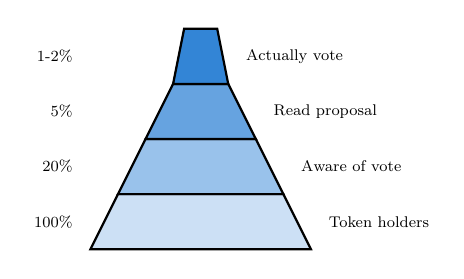
\begin{tikzpicture}[scale=0.7, transform shape]
% Participation funnel
\draw[thick, fill=dfblue!20] (0,0) -- (4,0) -- (3.5,1) -- (0.5,1) -- cycle;
\draw[thick, fill=dfblue!40] (0.5,1) -- (3.5,1) -- (3,2) -- (1,2) -- cycle;
\draw[thick, fill=dfblue!60] (1,2) -- (3,2) -- (2.5,3) -- (1.5,3) -- cycle;
\draw[thick, fill=dfblue!80] (1.5,3) -- (2.5,3) -- (2.3,4) -- (1.7,4) -- cycle;

\node[right, font=\footnotesize] at (4.2,0.5) {Token holders};
\node[right, font=\footnotesize] at (3.7,1.5) {Aware of vote};
\node[right, font=\footnotesize] at (3.2,2.5) {Read proposal};
\node[right, font=\footnotesize] at (2.7,3.5) {Actually vote};

\node[left, font=\footnotesize] at (-0.2,0.5) {100\%};
\node[left, font=\footnotesize] at (-0.2,1.5) {20\%};
\node[left, font=\footnotesize] at (-0.2,2.5) {5\%};
\node[left, font=\footnotesize] at (-0.2,3.5) {1-2\%};
\end{tikzpicture}
\end{column}
\end{columns}
\end{frame}

% =====================================================================
% SLIDE 27: Code is Law vs Rule of Law  [H44 FIXED --- mens rea defined; M9 cross-ref]
% =====================================================================
\begin{frame}{``Code is Law'' vs. Rule of Law}
\begin{columns}[T]
\begin{column}{0.48\textwidth}
\textbf{``Code is Law'' Philosophy:}
\begin{itemize}
\item Smart contract IS the agreement
\item No external intervention
\item Predictable, immutable
\item ``If the code allows it, it's allowed''
\end{itemize}

\vspace{3mm}
\textbf{The DAO Hack Challenge} (see slide 4):
\begin{itemize}
\item Hacker used code as designed
\item Was it theft or legitimate use?
\item Ethereum community chose to fork
\item ``Code is law'' violated by humans
\end{itemize}
\end{column}
\begin{column}{0.48\textwidth}
\textbf{Traditional Rule of Law:}
\begin{itemize}
\item Intent matters---\textit{mens rea} (Latin: ``guilty mind,'' the legal concept that you must intend to do wrong to be criminally liable)
\item Fairness considerations
\item Courts interpret disputes
\item Law evolves with society
\end{itemize}

\vspace{3mm}
\begin{alertblock}{The Tension}
Code cannot encode intent, fairness, or context. Pure ``code is law'' may be unjust. But human intervention undermines decentralization.
\end{alertblock}
\end{column}
\end{columns}
\end{frame}

% =====================================================================
% SLIDE 28: Hands-On Exercise Introduction  [M7 FIXED --- reduced to 3 exercises]
% =====================================================================
\begin{frame}{Hands-On: DAO Voting Simulation (NB12)}
\begin{center}
\textbf{\Large Model How Token Distribution Affects Governance}
\end{center}

\vspace{5mm}
\textbf{In the Colab notebook, we will:}
\begin{enumerate}
\item Create token distributions with varying concentration and simulate voting on proposals ($\sim$8 min)
\item Test attack scenarios: whale dominance and flash loans ($\sim$7 min)
\item Explore defense mechanisms: quadratic voting, delegation ($\sim$7 min)
\end{enumerate}

\vspace{5mm}
\begin{block}{Access the Notebook}
\texttt{day\_05/notebooks/NB12\_dao\_governance\_simulation.ipynb}

\vspace{2mm}
\footnotesize See how 1 whale with 51\% can override 10,000 small holders.
\end{block}

\bottomnote{Time: 20--25 minutes for guided exploration}
\end{frame}

% =====================================================================
% SLIDE 29: Hands-On Exercise Details
% =====================================================================
\begin{frame}{NB12: Key Simulation Exercises}
\begin{columns}[T]
\begin{column}{0.48\textwidth}
\textbf{Exercise 1: Distribution \& Voting}
\begin{itemize}
\item Generate realistic Pareto distributions
\item Visualize wealth concentration
\item Calculate Gini coefficient
\item Simulate proposal voting
\item Model whale vs.\ community outcomes
\end{itemize}

\vspace{3mm}
\textbf{Exercise 2: Attack Scenarios}
\begin{itemize}
\item Model flash loan attack
\item Test vote buying economics
\item Simulate 51\% accumulation
\item Measure attack costs
\end{itemize}
\end{column}
\begin{column}{0.48\textwidth}
\textbf{Exercise 3: Defense Mechanisms}
\begin{itemize}
\item Implement quadratic voting
\item Test conviction voting
\item Model delegation effects
\item Compare outcomes across mechanisms
\end{itemize}

\vspace{3mm}
\begin{block}{Key Question to Answer}
How does changing from 1-token-1-vote to quadratic voting affect a whale's ability to pass self-serving proposals?
\end{block}
\end{column}
\end{columns}
\end{frame}

% =====================================================================
% SLIDE 30: Discussion - Governance Tradeoffs  [H49 FIXED --- trilemma expanded]
% =====================================================================
\begin{frame}{Discussion: Governance Tradeoffs}
\begin{columns}[T]
\begin{column}{0.48\textwidth}
\textbf{Questions to Consider:}
\begin{enumerate}
\item Is plutocracy inherent to token voting?
\item Should DAOs have constitutions?
\item When is centralization acceptable?
\item Can code ever fully replace human judgment?
\end{enumerate}

\vspace{2mm}
\textbf{Key Takeaways:}
\begin{itemize}
\item Governance IS the attack surface
\item Token distribution = power distribution
\item ``Decentralized'' often isn't
\item Hybrid models emerging
\end{itemize}
\end{column}
\begin{column}{0.48\textwidth}
\begin{alertblock}{The Governance Trilemma}
You can optimize for two of three: \textbf{Decentralization}, \textbf{Efficiency}, \textbf{Security}. Pick which one to sacrifice.
\end{alertblock}

\vspace{2mm}
\textbf{Examples:}
\begin{itemize}
\item \textbf{Company board} = efficient + secure, but centralized
\item \textbf{Bitcoin governance} = decentralized + secure, but slow (years to change)
\item \textbf{Small DAO with optimistic voting} = decentralized + efficient, but vulnerable to attacks
\end{itemize}
\end{column}
\end{columns}
\end{frame}

% =====================================================================
% SLIDE 31: Application - Real DAO Examples (Part 1)
%   [M3, M4 FIXED --- Curve gauge/wars explained; split from 12-item slide M8]
% =====================================================================
\begin{frame}{Application: Real DAO Governance Examples (1/2)}
\begin{columns}[T]
\begin{column}{0.48\textwidth}
\textbf{MakerDAO:}
\begin{itemize}
\item Governs DAI stablecoin
\item MKR token for voting
\item Complex risk parameters
\item Executive votes for changes
\end{itemize}

\vspace{3mm}
\textbf{Uniswap:}
\begin{itemize}
\item UNI token governance
\item 7-day timelock
\item 4\% quorum requirement
\item Treasury grants program
\end{itemize}
\end{column}
\begin{column}{0.48\textwidth}
\textbf{Compound:}
\begin{itemize}
\item COMP token governance
\item On-chain proposals
\item 48-hour timelock
\item Delegation system
\end{itemize}

\vspace{3mm}
\textbf{Aave:}
\begin{itemize}
\item AAVE token governance
\item Two-tier proposal system
\item Progressive decentralization
\item Cross-chain governance emerging
\end{itemize}
\end{column}
\end{columns}
\end{frame}

% =====================================================================
% SLIDE 32: Application - Real DAO Examples (Part 2)  [M3, M4, M8 FIXED]
% =====================================================================
\begin{frame}{Application: Real DAO Governance Examples (2/2)}
\begin{columns}[T]
\begin{column}{0.48\textwidth}
\textbf{Curve Finance:}
\begin{itemize}
\item veCRV model pioneer (lock tokens for votes)
\item Up to 4-year locks
\item \textbf{Gauge voting for emissions:} token holders vote on which liquidity pools receive newly minted CRV rewards each week --- controlling where incentives flow
\item \textbf{``Curve Wars'':} DAOs competing to accumulate veCRV so they can direct CRV rewards to their own pools --- a battle for governance power over the largest stablecoin exchange
\end{itemize}
\end{column}
\begin{column}{0.48\textwidth}
\textbf{Why Curve Wars Matter:}

The Curve Wars illustrate a key governance insight: when governance tokens control real economic flows (like reward emissions worth millions per week), governance power itself becomes a valuable asset that other protocols will fight to acquire.

\vspace{3mm}
\begin{block}{Pattern}
Governance power $\rightarrow$ economic control $\rightarrow$ arms race for governance tokens $\rightarrow$ further concentration.
\end{block}
\end{column}
\end{columns}
\end{frame}

% =====================================================================
% SLIDE 33: Application - DAO Design Considerations
% =====================================================================
\begin{frame}{Application: Designing DAO Governance}
\begin{columns}[T]
\begin{column}{0.48\textwidth}
\textbf{Key Design Questions:}
\begin{enumerate}
\item Who can submit proposals?
\item What is the voting period?
\item What quorum is required?
\item How long is the timelock?
\item Who has veto power?
\end{enumerate}

\vspace{3mm}
\textbf{Progressive Decentralization:}
\begin{itemize}
\item Start with strong team control
\item Gradually add community power
\item Remove training wheels over time
\item Earn trust through track record
\end{itemize}
\end{column}
\begin{column}{0.48\textwidth}
\textbf{Common Governance Stack:}
\begin{enumerate}
\item \textbf{Forum:} Discussion (Discourse)
\item \textbf{Signaling:} Temperature check (Snapshot)
\item \textbf{Voting:} Binding vote (Governor)
\item \textbf{Execution:} Timelock controller
\item \textbf{Safety:} Guardian multi-sig
\end{enumerate}

\vspace{3mm}
\begin{block}{OpenZeppelin Governor}
Standard, audited implementation covering the full governance lifecycle.
\end{block}
\end{column}
\end{columns}
\end{frame}

% =====================================================================
% SLIDE 34: Application - Future of DAO Governance
%   [M2, L1, L2 FIXED --- futarchy, soulbound, non-US legal]
% =====================================================================
\begin{frame}{Application: The Future of DAO Governance}
\begin{columns}[T]
\begin{column}{0.48\textwidth}
\textbf{Emerging Innovations:}
\begin{itemize}
\item \textbf{Reputation-based voting:} Non-transferable credentials
\item \textbf{Soulbound tokens:} Identity-linked voting power (named after non-transferable items in video games --- once earned, they cannot be sold or given away)
\item \textbf{Futarchy:} Governance by prediction markets --- bet on outcomes to decide policy. If the market predicts Policy A leads to better results, Policy A wins
\item \textbf{AI governance:} Automated analysis of proposals
\end{itemize}
\end{column}
\begin{column}{0.48\textwidth}
\textbf{Legal Developments:}
\begin{itemize}
\item Wyoming DAO LLC law (USA)
\item Marshall Islands DAO recognition
\item EU MiCA framework (Europe)
\item Switzerland's ``DLT Act'' (enables tokenized securities and DAO-like structures)
\item Regulatory clarity emerging globally
\end{itemize}

\vspace{3mm}
\begin{block}{Open Question}
Can DAOs become the dominant organizational form of the 21st century, or are they limited to niche applications where trust minimization is paramount?
\end{block}
\end{column}
\end{columns}
\end{frame}

% =====================================================================
% SLIDE 35: Executive Summary
% =====================================================================
\begin{frame}{Executive Summary}
\begin{columns}[T]
\begin{column}{0.48\textwidth}
\textbf{Core Concepts:}
\begin{enumerate}
\item DAOs encode governance in smart contracts
\item Token-based voting creates plutocracy
\item Quadratic voting reduces but doesn't eliminate whale power
\item Flash loans can exploit instant-execution governance
\item Timelocks and snapshots are essential defenses
\end{enumerate}
\end{column}
\begin{column}{0.48\textwidth}
\textbf{Key Insights:}
\begin{enumerate}
\item Governance IS the attack surface
\item ``Decentralized'' is often a spectrum
\item Voter apathy is rational behavior
\item Code cannot encode fairness
\item Hybrid models work best
\end{enumerate}
\end{column}
\end{columns}

\vspace{5mm}
\begin{block}{One-Sentence Summary}
DAO governance attempts to solve collective decision-making without trusted intermediaries, but faces fundamental tradeoffs between decentralization, efficiency, and security that make true ``decentralization'' elusive in practice.
\end{block}
\end{frame}

% =====================================================================
% SLIDE 36: Concept Map
% =====================================================================
\begin{frame}{Concept Map: DAO Governance}
\begin{center}
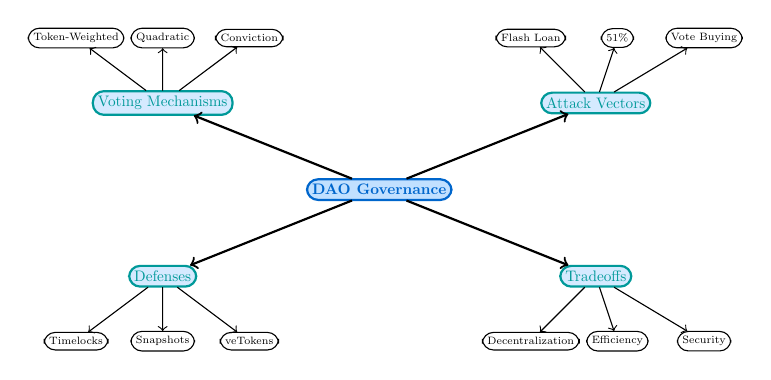
\begin{tikzpicture}[scale=0.55, transform shape]
% Central node
\node[draw, thick, dfblue, fill=dflightblue3, rounded corners, minimum width=2cm] (dao) at (0,0) {\textbf{DAO Governance}};

% Level 1
\node[draw, thick, dfteal, fill=dflightblue4, rounded corners] (voting) at (-5,2) {Voting Mechanisms};
\node[draw, thick, dfteal, fill=dflightblue4, rounded corners] (attacks) at (5,2) {Attack Vectors};
\node[draw, thick, dfteal, fill=dflightblue4, rounded corners] (defenses) at (-5,-2) {Defenses};
\node[draw, thick, dfteal, fill=dflightblue4, rounded corners] (tradeoffs) at (5,-2) {Tradeoffs};

% Level 2 - Voting
\node[draw, rounded corners, font=\scriptsize] (token) at (-7,3.5) {Token-Weighted};
\node[draw, rounded corners, font=\scriptsize] (quadratic) at (-5,3.5) {Quadratic};
\node[draw, rounded corners, font=\scriptsize] (conviction) at (-3,3.5) {Conviction};

% Level 2 - Attacks
\node[draw, rounded corners, font=\scriptsize] (flash) at (3.5,3.5) {Flash Loan};
\node[draw, rounded corners, font=\scriptsize] (vote51) at (5.5,3.5) {51\%};
\node[draw, rounded corners, font=\scriptsize] (bribe) at (7.5,3.5) {Vote Buying};

% Level 2 - Defenses
\node[draw, rounded corners, font=\scriptsize] (timelock) at (-7,-3.5) {Timelocks};
\node[draw, rounded corners, font=\scriptsize] (snapshot) at (-5,-3.5) {Snapshots};
\node[draw, rounded corners, font=\scriptsize] (vetoken) at (-3,-3.5) {veTokens};

% Level 2 - Tradeoffs
\node[draw, rounded corners, font=\scriptsize] (decent) at (3.5,-3.5) {Decentralization};
\node[draw, rounded corners, font=\scriptsize] (effic) at (5.5,-3.5) {Efficiency};
\node[draw, rounded corners, font=\scriptsize] (secure) at (7.5,-3.5) {Security};

% Connections
\draw[->, thick] (dao) -- (voting);
\draw[->, thick] (dao) -- (attacks);
\draw[->, thick] (dao) -- (defenses);
\draw[->, thick] (dao) -- (tradeoffs);

\draw[->] (voting) -- (token);
\draw[->] (voting) -- (quadratic);
\draw[->] (voting) -- (conviction);

\draw[->] (attacks) -- (flash);
\draw[->] (attacks) -- (vote51);
\draw[->] (attacks) -- (bribe);

\draw[->] (defenses) -- (timelock);
\draw[->] (defenses) -- (snapshot);
\draw[->] (defenses) -- (vetoken);

\draw[->] (tradeoffs) -- (decent);
\draw[->] (tradeoffs) -- (effic);
\draw[->] (tradeoffs) -- (secure);
\end{tikzpicture}
\end{center}
\end{frame}

% =====================================================================
% SLIDE 37: Key Terms (Part 1)
% =====================================================================
\begin{frame}{Key Terms (1/2)}
\begin{columns}[T]
\begin{column}{0.48\textwidth}
\textbf{DAO:} Decentralized Autonomous Organization---rules encoded in smart contracts, decisions via token voting.

\vspace{2mm}
\textbf{Governance Token:} Token representing voting power in organizational decisions.

\vspace{2mm}
\textbf{Token-Weighted Voting:} 1 token = 1 vote system; simple but plutocratic.

\vspace{2mm}
\textbf{Quadratic Voting:} Voting power = $\sqrt{\text{tokens}}$; reduces whale influence.

\vspace{2mm}
\textbf{Conviction Voting:} Voting power accumulates over time; rewards long-term alignment.
\end{column}
\begin{column}{0.48\textwidth}
\textbf{Delegation:} Lending voting power to trusted representatives while retaining token ownership.

\vspace{2mm}
\textbf{Quorum:} Minimum participation threshold for valid vote.

\vspace{2mm}
\textbf{Timelock:} Delay between proposal approval and execution; security mechanism.

\vspace{2mm}
\textbf{Snapshot Voting:} Using historical token balance for voting power; prevents flash loan attacks.

\vspace{2mm}
\textbf{veToken:} Vote-escrowed token; locked tokens for increased voting power.
\end{column}
\end{columns}
\end{frame}

% =====================================================================
% SLIDE 38: Key Terms (Part 2)
% =====================================================================
\begin{frame}{Key Terms (2/2)}
\begin{columns}[T]
\begin{column}{0.48\textwidth}
\textbf{Flash Loan Attack:} Borrowing tokens temporarily to vote on malicious proposals.

\vspace{2mm}
\textbf{51\% Attack:} Accumulating majority tokens to control all governance decisions.

\vspace{2mm}
\textbf{Vote Buying:} Paying token holders (directly or via protocols) to vote a certain way.

\vspace{2mm}
\textbf{Plutocracy:} Rule by the wealthy; inherent risk in token-weighted voting.

\vspace{2mm}
\textbf{Voter Apathy:} Low participation due to costs, complexity, or rational ignorance.
\end{column}
\begin{column}{0.48\textwidth}
\textbf{Multi-Sig:} N-of-M signature requirement; used for treasury management.

\vspace{2mm}
\textbf{Guardian:} Trusted entity with veto power for emergency situations.

\vspace{2mm}
\textbf{Sybil Attack:} One person creating many fake identities to gain disproportionate influence.

\vspace{2mm}
\textbf{On-Chain Governance:} Voting and execution happen on blockchain; automatic but costly.

\vspace{2mm}
\textbf{Off-Chain Governance:} Voting off-chain (e.g., Snapshot); free but requires manual execution.

\vspace{2mm}
\textbf{Code is Law:} Philosophy that smart contract code defines all valid behavior.
\end{column}
\end{columns}
\end{frame}

% =====================================================================
% SLIDE 39: Common Misconceptions
% =====================================================================
\begin{frame}{Common Misconceptions}
\begin{columns}[T]
\begin{column}{0.48\textwidth}
\textbf{Misconception 1:}\\
``DAOs are truly decentralized''

\textbf{Reality:} Token concentration means a few wallets often control outcomes. Most DAOs are plutocracies in practice.

\vspace{4mm}
\textbf{Misconception 2:}\\
``1 token = 1 vote is fair''

\textbf{Reality:} It's fair by one definition (stake-weighted), but it gives wealthy holders disproportionate control over protocol direction.

\vspace{4mm}
\textbf{Misconception 3:}\\
``Quadratic voting solves whale dominance''

\textbf{Reality:} Without identity systems, whales simply split tokens across wallets to game quadratic voting (Sybil attack).
\end{column}
\begin{column}{0.48\textwidth}
\textbf{Misconception 4:}\\
``Code is law provides certainty''

\textbf{Reality:} Code cannot encode intent, context, or fairness. Communities regularly intervene when code produces unjust outcomes.

\vspace{4mm}
\textbf{Misconception 5:}\\
``High quorum prevents attacks''

\textbf{Reality:} High quorum can make governance non-functional. Attackers with sufficient tokens can still reach quorum.

\vspace{4mm}
\textbf{Misconception 6:}\\
``Token holders = users''

\textbf{Reality:} Many token holders are speculators; actual protocol users may have no governance voice.
\end{column}
\end{columns}
\end{frame}

% =====================================================================
% SLIDE 40: Self-Assessment Questions (Part 1)
% =====================================================================
\begin{frame}{Self-Assessment Questions (1/2)}
\textbf{Question 1:} What does DAO stand for in blockchain governance?

\vspace{2mm}
\begin{enumerate}[A.]
\item Distributed Autonomous Operation
\item Decentralized Autonomous Organization
\item Digital Asset Organization
\item Delegated Authority Operation
\end{enumerate}

\vspace{5mm}
\textbf{Question 2:} What happens when you delegate your governance tokens?

\vspace{2mm}
\begin{enumerate}[A.]
\item You permanently transfer ownership
\item The delegate can vote with your voting power on your behalf
\item Your tokens are locked and cannot be moved
\item You lose all rights until delegation is revoked
\end{enumerate}

\vspace{5mm}
\footnotesize\textit{Answers: 1-B, 2-B}
\end{frame}

% =====================================================================
% SLIDE 41: Self-Assessment Questions (Part 2)
% =====================================================================
\begin{frame}{Self-Assessment Questions (2/2)}
\textbf{Question 3:} What is the most effective defense against flash loan governance attacks?

\vspace{2mm}
\begin{enumerate}[A.]
\item Requiring voters to stake tokens for the entire voting period
\item Increasing gas costs for voting transactions
\item Using snapshot voting power from before proposal creation
\item Limiting tokens that can participate in any proposal
\end{enumerate}

\vspace{5mm}
\textbf{Reflection Questions:}
\begin{itemize}
\item Can true decentralization exist with token-weighted voting?
\item How would you design governance that balances efficiency and security?
\item What role should human judgment play in ``code is law'' systems?
\end{itemize}

\vspace{3mm}
\footnotesize\textit{Answer: 3-C (Snapshot voting captures historical balance, making flash loans ineffective since attacker had 0 balance at snapshot)}
\end{frame}

% =====================================================================
% SLIDE 42: What's Next
% =====================================================================
\begin{frame}{What's Next: Topic 5.4 -- Privacy and Financial Inclusion}
\begin{columns}[T]
\begin{column}{0.48\textwidth}
\textbf{Preview of T5.4:}
\begin{itemize}
\item Blockchain transparency vs. privacy
\item Surveillance capabilities and risks
\item Privacy-preserving technologies
\item Zero-knowledge proofs basics
\item Financial inclusion opportunities
\end{itemize}

\vspace{3mm}
\textbf{Connection to DAO Governance:}\\
Privacy tools could enable anonymous voting, reducing vote buying and social pressure.
\end{column}
\begin{column}{0.48\textwidth}
\textbf{Key Questions for T5.4:}
\begin{enumerate}
\item Is blockchain transparency a feature or bug?
\item How do privacy coins work?
\item Can DeFi serve the unbanked?
\item What are ZK-proofs and why do they matter?
\end{enumerate}

\vspace{3mm}
\begin{block}{Prepare}
Consider: How does the public nature of blockchain transactions affect governance participation? Would you vote differently if your vote was anonymous?
\end{block}
\end{column}
\end{columns}
\end{frame}

% =====================================================================
% SLIDE 43: Resources
% =====================================================================
\begin{frame}{Resources for Further Learning}
\begin{columns}[T]
\begin{column}{0.48\textwidth}
\textbf{Academic Papers:}
\begin{itemize}
\item Buterin et al., ``Liberal Radicalism'' (Quadratic Voting)
\item Weyl \& Posner, ``Radical Markets''
\item Catalini \& Gans, ``Initial Coin Offerings''
\end{itemize}

\vspace{3mm}
\textbf{Technical Documentation:}
\begin{itemize}
\item OpenZeppelin Governor docs
\item Compound Governance whitepaper
\item Snapshot documentation
\item Curve veToken mechanics
\end{itemize}
\end{column}
\begin{column}{0.48\textwidth}
\textbf{Case Studies:}
\begin{itemize}
\item The DAO hack (2016)
\item Beanstalk attack (2022)
\item MakerDAO governance evolution
\item Curve Wars analysis
\end{itemize}

\vspace{3mm}
\textbf{Tools to Explore:}
\begin{itemize}
\item Tally (governance aggregator)
\item DeepDAO (DAO analytics)
\item Boardroom (governance dashboards)
\item Snapshot.org (off-chain voting)
\end{itemize}
\end{column}
\end{columns}

\vspace{3mm}
\begin{block}{Hands-On Practice}
\texttt{day\_05/notebooks/NB12\_dao\_governance\_simulation.ipynb}
\end{block}
\end{frame}

% =====================================================================
% SLIDE 44: Questions?
% =====================================================================
\begin{frame}{Questions?}
\begin{center}
\vspace{10mm}
{\Huge Questions?}

\vspace{15mm}
\textbf{Topic 5.3: DAO Governance}\\
Decentralized Autonomous Organizations

\vspace{10mm}
\textit{``Governance is the attack surface.''}

\vspace{10mm}
\small
Joerg Osterrieder\\
Digital Finance\\
2025
\end{center}
\end{frame}

\end{document}
